\subsection{Overview}

\todo{make this actually an overview}

The second part of this project was focused on producing a library of HSL analogue-ciprofloxacin conjugates. The HSL head group was replaced with a selection of cyclic amines found in known quorum sensing modulators (see \ref{sec:AIA_intro}). The analogues were linked to ciprofloxacin in two ways: using a copper(I)-catalysed azide-alkyne cycloaddition\cite{Tornoe2002,ANIE:ANIE2596} with the alkynyl ciprofloxacin derivative \compound{cmpd:Y4Cip} synthesised in \ref{sec:Y4Cip} and directly using either an S$_N$2 reaction or peptide coupling.




\subsubsection{Head groups}

The head groups used in this study are shown in \ref{fig:head_groups}. The cyclohexanol derivatives were synthesised as a diastereomerically pure racemate, whereas the cyclopentanol derivatives were synthesised as separate enantiomers. Unfortuantely, cyclopentanone derivatives were not synthesised, and would be an obvious future addition to the library. The 2-methoxybenzene derivatives do not have precedents as quorum sensing modulators in the literature, but they were included so as to be compared with the 3-methoxybenzene derivatives.

\begin{figure}[H]
	\begin{center}
		\includegraphics[scale=1]{head_groups}
		\caption{The head groups used in this section.\label{fig:head_groups}}
	\end{center}
\end{figure}

\subsubsection{Library construction}

As Ganguly \textit{et al.}\cite{Ganguly2001} synthesised their conjugate from Br-C$_4$-HCTL, it was envisaged that a branching strategy could be used to produce two sets of conjugates (see \ref{sch:branching_synth_general}). The first set would be formed by the S$_N$2 reaction of the relevant bromide with methyl ciprofloxacin. The second set would be made by displacing the bromide with azide, then performing a click reaction with the alkynyl ciprofloxacin derivative \compound{cmpd:Y4Cip} made previously to form the triazole-linked product. Ketone conjugates would be formed by oxidation of the alcohols.

\begin{scheme}[H]
	\begin{center}
		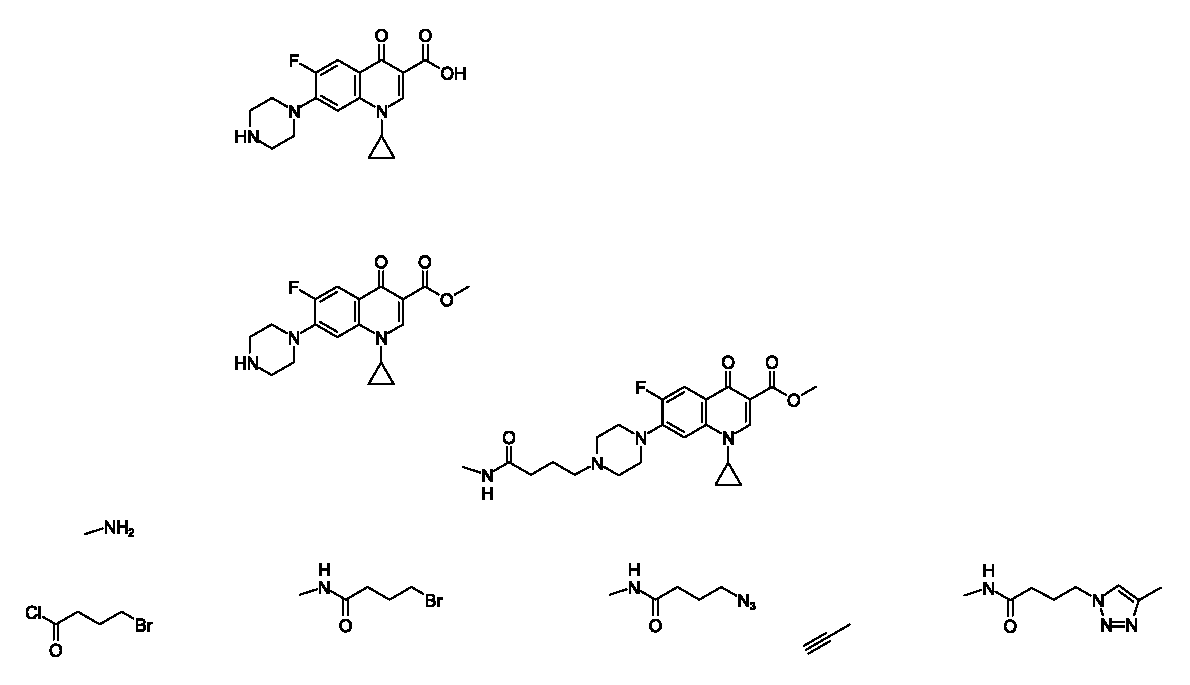
\includegraphics[scale=1]{branching_synth_general}
		\caption{\label{sch:branching_synth_general}}
	\end{center}
\end{scheme}

